\chapter{Solution}
\label{solution}

\section{Design and Planning of learning process}

http://www.teaching.utoronto.ca/topics/coursedesign/learning-outcomes/outcomes-objectives.htm




The Design phase contains three steps: First Design Assessments, second choose a course format, third create an instructional strategy.

Design assessments before creating a content - nagu tagant ettepoole minek.



\subsubsection{Analysis of the course content}
All times are given in academic hours or days which equal 8 academic hours.
\begin{enumerate}[label=Hands-on block \arabic*.,leftmargin=*]
  \item Pre-requirements courses
    \begin{enumerate}[label=LAB \arabic*.,leftmargin=*]
  	\item Operating system basics (one day)
  	\item Basic networking IPv4/IPv6, TCP/IP (one day)
  	\item GNU/Linux basics (and OpenBSD/FreeBSD basics) (16h) as describbed in Appendix~\ref{Preliminary course - dpkg based GNU/Linux} on page~\pageref{Preliminary course - dpkg based GNU/Linux}
  	\item Scripting in BASH (2 days)
  	\item Scripting in Python (1.5 days)
  	\item Scripting in PowerShell (1.5 days)
  \end{enumerate}
  \item Root services
  \begin{enumerate}[label=LAB \arabic*.,leftmargin=*]
  	\item NTP (0.5 days)
  	\item DNS (2.5 days)
  	\item DHCP (one day)
  \end{enumerate}
  \item Web/File Services
    \begin{enumerate}[label=LAB \arabic*.,leftmargin=*]
    \item Web server basics - installation of apache2 web server
  	\item Web server security - Protecting Web Application Against
(D)DOS Attacks
  	\item Web server security - securing vulnerable web application using application firewalls (3 days)
  	\item Fileserver (Samba3 and Samba4) (0.5 day)
  \end{enumerate}
    \item E-mail services (4 days)
    \begin{enumerate}[label=LAB \arabic*.,leftmargin=*]
  		\item SPAM control
	  	\item Virus protection
  		\item MTA's 
	  	\item MDA's
    \end{enumerate}
    \item IP firewalls and IDS/IPS (4 days)
        \begin{enumerate}[label=LAB \arabic*.,leftmargin=*]
  		\item IP firewalls netfilter/iptables and packet filter (pf) (2 days)
	  	\item IDS/IPS (2 days)
  		\item NetFlow (kuna seda loetakse CERT.EE abil, siis jääb välja)
    \end{enumerate}
    \item Autentication and authorization (4 days)
        \begin{enumerate}[label=LAB \arabic*.,leftmargin=*]
  		\item LDAP and Samba4 AD
	  	\item Windows and Linux clients with Samba4 AD 
  		\item Web application authentication with Samba4 AD and LDAP
    		\end{enumerate}
    \item GNU/Linux central management with Puppet
        \begin{enumerate}[label=LAB \arabic*.,leftmargin=*]
	  		\item Installation of Puppet using passenger (2 day)
		  	\item Writing puppet recipes (1 day)
    		\end{enumerate}
    	\item Central logging (3 days)
    	    \begin{enumerate}[label=LAB \arabic*.,leftmargin=*]
	  		\item Collecting logs with rsyslog/syslog-ng (1 day)
		  	\item Monitor and analyse log files (1 day)
    		\end{enumerate}
\end{enumerate}


Assessment design contains (goals, lerners, context, assessment)
kõiki õpiväljundeid tuleb testida.
assessments: clearly written, correct punctuation and grammar.

Choosing a course format is a delivery system like medium used to present the course.
- classroom
- e-course
- blended -combines different methods
- 

Instructional strategy
Collection of 
-lectures
-readings
-discussions
-projects
-worksheets
-assessments
-activities
Activities can be divided into five topics
\begin{enumerate}
\item Pre-instructional activities (motivate the students, mida nad pärast paremini teha oskavad, peale seda presenteerida objectives)
\item Content Presentation (consice content - no too many details, examples, )
\item Learner Participation (practice and feedback, )
\item Assessment (lisaks final assesment, practical assesment, attitude assesment  - ask students how thei feel about course )
\item Follow-through activities (review of entire course strategy .. veidi segane)
\end{enumerate}



Two possible e-learning processes are common the self-paced and facilitated/instructor-led \citep[p.~10]{food2011learning}.

Do we use collaboration in learning? 

Do we use  e-tutoring, e-coaching, e-mentoring?

Do we use chronological order or problem based? (one is good for lecturing other for practical classes) Also possible ways is spiral order logical order etc {\color{red} (viidata) }

Is the content sufficient to gain learning outcomes?

Is amount of work and student workload normal? How many academic hours for practical classes and home reading/lectures?

\subsection{Pedagogical view of the e-course}
Different Pedagogical strategies can be used during learning process. First a problem based approach is {\color{red} Pooleli }
Second koostööl põhinev õpe ja kolmas kogukonnal põhinev õpe.

Do we use group-work, wiki, blog and/or some e-learning environment?

Synchronous or asynchronous learning.

\subsection{Planning grading/assessment techniques}
What grading methods are useful for this particular course?

Do we need grade knowledge, skills and {\color{red} Pooleli }

Several assessment methods are used to give feedback and grades for students in e-courses {\color{red} Viide+listile viide }

\begin{itemize}
	\item self-assessment
	\item computer assessment
	\item tutor assessment
	\item peer assessment
\end{itemize}
\subsection{Choosing technological tools}
Keywords to focus {\color{red} Viidata }
\begin{itemize}
	\item availability
	\item usability 
	\item motivating students
	\item adaptive methods
	\item standard compliance
\end{itemize}
\subsubsection{E-Learning platforms}

\begin{itemize}
	\item Millal e-õpe töötab ja millal ei? Õppur peab rohkem pingutama [Chao: 11]
	\item Erinevad õpikeskkonnad ja nende sobivus antud õppeks
		\begin{itemize}
			\item Moodle
			\item Blackboard WebCT
			\item CISCO Network Academy
			\item Maurus
			\item IVA
			\item Sakai
			\item Wikiversity
			\item TUT Kaur course lab
		\end{itemize}
	\item virtual distance laboratory
	\item security aspects of distance laboratory
\end{itemize}






Õpiväljundid on mõeldud õppijate jaoks, et anda neile ülevaade sellest, mida kursuselt oodata ning
millele selle jooksul rõhku panna. Sellest lähtuvalt tuleks nad ka sõnastada vastavalt, st mitte õpetaja
vaid just õppijakeskselt, kirjeldades mitte seda, mis toimub kursuse käigus vaid keskendudes sellele,
mida uut peaks õppija suutma teha kursuse lõpuks.

\begin{enumerate}[label=Learning Objective \arabic*.,leftmargin=*]
\item NTP, DNS ,DHCP
\item Web server, OWASP, DVWA,
\item VPN, SAN, NAS, IDS, IPS
\end{enumerate}





\begin{enumerate}
\item Create a Sample (see on kliendile, testiks ja prototüübiks)
\item Develop the course Materials (peab teadma activities + tagasiside review)
\item Conduct a Run-through (real-time rehearsal testi sõbra peal kogu kursust +  feedback assessment + saab reaalselt teada aja, mis kulub kursuse läbimisele
\end{enumerate}


The implementation phase of the ADDIE Model contains three sub-phases

\begin{enumerate}
\item Train the Instructor
\item Prepare the Learners
\item Arrange the Learning Space
\end{enumerate}

Train the Instructor - course developer is often a trainer too but some cases you need more people to train


Development:
Authoring
Media creation / integration / production
Prototyping
Processing
Quality Assurance

\section{Development of the e-learning course}

\subsection{Authoring the learning material}
In the development phase the authoring of learning materials, tests, media and integration of all artefacts into consistent body. 

\url{http://www.grayharriman.com/ADDIE.htm}

\begin{table}[h]
\centering
\caption{The learning materials}

\begin{tabular}{|p{5cm}|p{3cm}|p{6cm}|}
\hline 
\color{blue}
Name & \color{blue} Comments  & \color{blue} Location \\ 

\hline
  \multicolumn{3}{|c|}{Pre-requirement course} \\
\hline
Operating system basics & & \\
\hline
Basic networking IPv4/IPv6, TCP/IP & & \\

\hline
GNU/Linux basics (and OpenBSD/FreeBSD basics)  & & \\
\hline
Scripting in BASH &  & \\
\hline
Scripting in Python & Co authored with Lauri Võsandi & \\
\hline
Scripting in PowerShell & Author is Heiki Tähis & \\


\hline
\hline
  \multicolumn{3}{|c|}{Root services} \\

\hline 


Lecture - Configuring NTP service & (Estonian 2012), Learning outcome no XXX & \url{http://goo.gl/toRpw} \\ 
\hline 
Practical class - Configuring NTP in Ubuntu  & (Estonian 2012), Learning outcome no XXX , Students improved & \url{https://wiki.itcollege.ee/index.php/NTP_Ubuntus} \\
\hline 
Lecture DNS & & \href{http://enos.itcollege.ee/~mernits/infrastruktuur/Interneti%20domeeninimede%20s%c3%bcsteem%20-%20IT%20infra%20loeng.odp}
{DNS Lecture [OpenDocument]} \\
\hline
Practical class - DNS & Co authored with Katrin Loodus  & \href{https://docs.google.com/document/d/1ZeQpPXdVq1C7RQpxQYR0gBB0OBMYB_0g6aFFxs_-fIA/edit}{Configuring DNS [GoogleDocs] } \\

\hline
\hline
  \multicolumn{3}{|c|}{Web/File Services} \\

\hline 
 & & \\
\hline

\hline
 & & \\
\hline
\hline
  \multicolumn{3}{|c|}{E-mail service} \\
\hline 
 & & \\
\hline

\hline
 & & \\

\hline
\hline
  \multicolumn{3}{|c|}{IP firewalls and IDS/IPS} \\
\hline 
 & & \\
\hline

\hline
 & & \\

\hline
\hline
  \multicolumn{3}{|c|}{Autentication and authorization} \\
\hline 
 & & \\
\hline

\hline
 & & \\

\hline
 & & \\
\hline
\end{tabular} 
\label{table:learning_materials}
\end{table}


\subsection{Text based learning material}
Developed learning material should follow consistent style and present also one example of good documentation practice. For system administrators several howto styles exists. However practical hands-on laboratory instructions are designed that pass through using copy paste is possible but gives one working sample. However, this is not enough to pass lab scenario and student must customize own configuration.

Guiding stile of the lab instruction using style convention: First, all variable parts of the text are clearly differs from other text and command. Second, all commands given by student are highlighted, and variable parts embossed as seen in followed command.


\begin{minted}[frame=lines,framesep=2mm]{bash}
#Sample for changing OOM adjustment score for mysql server
echo "-17" > /proc/$(pidof mysqld)/oom_adj
\end{minted}
%$


Sample sample: Finding a proccess ID of the mysql server proccess.

\begin{minted}[frame=lines,framesep=2mm]{bash}
ps -ef|grep mysqld
\end{minted}
\label{code_sample}
%
\small{
\begin{Verbatim}[frame=single,
label=Command output,framesep=2mm,rulecolor=\color{red},commandchars=\\\{\}]
sudent@opiise:~# ps -ef|grep mysqld
root     11290 10905  0 10:27 pts/6    00:00:00 grep --color=auto mysqld
mysql    \fbox{\color{red}29830}    1  0 Apr25 ?        00:05:47 /usr/sbin/mysqld
\end{Verbatim}
%
}

All study should stored in open formats, like pdf, OpenDocument , MediaWiki markup language, html, utf8 text. Original editable source files for generating pdf, images should be publicly accessible. Moreover, text based materials should stored into version control system like git or subversion to enable contributing for other lecturers and students as well.

\subsection{Audio/Visual learning material}
The Audio/Visual material is recorded from live lectures and practical classes using echo360 equipment or screen/audio recording for some classes. Recordings are supportive materials and not the main source for knowledge.

\url{http://echo360.e-uni.ee/ess/portal/section/36936084-4fbb-413c-98ec-0470f11db4e3}


\subsection{Interactive learning material}

\subsection{Online tests and laboratory scenarios}

\subsection{Learning objectives}

\subsection{Technical implementation of the e-course}

\LaTeX Minted muutujad jne


\subsubsection{The Environment of Distance Study}
\label{The Environment of Distance Study}
The Environment of Distance Study...

TODO pilt virtuaalaborite süsteemi kontekstist
\subsubsection{Random tags}
\begin{itemize}
	\item normal traffic generator
	\item malicious traffic generator
	\item availability monitor (for grading)
\end{itemize}

\subsubsection{Virtualization Layer}
Siin libvirdist
\subsubsection{Web Application Layer}
Siin Ruby on Rails raamistikust ja veebirakendusest
\subsubsection{Architecture of Distance Laboratory}
Siin räägin üldisest disainist ja allsüsteemidest
\
\begin{figure}[ht]
\centering
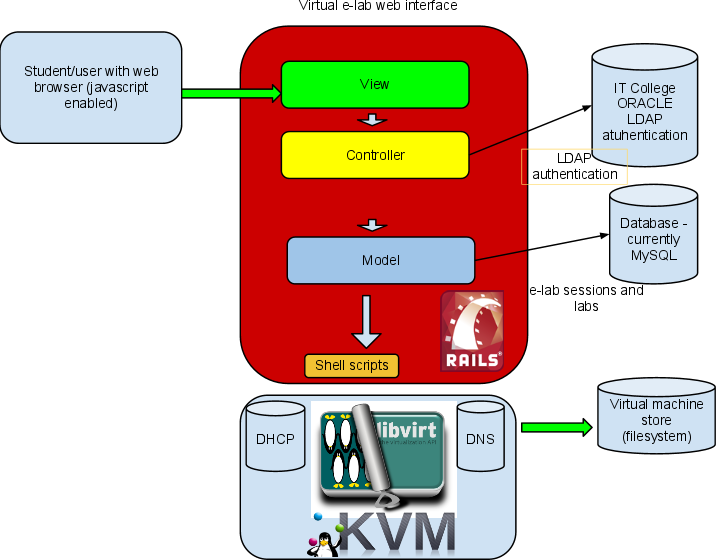
\includegraphics[width=0.8\textwidth]{architecture.png}
\caption{Architecture of Distance Laboratory}
\label{fig:Architecture of Distance Laboratory}
\end{figure}
\

\subsubsection{Security Aspects of Distance Laboratory}

\subsection{Testing the e-course}

\section{Piloting the course}

\subsection{Organizational role}

\subsection{Social role}

\subsection{Pedagogical role}